\documentclass[aspectratio=1610,t]{beamer}

\usepackage[english]{babel}
\usepackage{hyperref}
\usepackage{minted}
\usepackage{alltt}
\usepackage{amsmath}
\usepackage{graphicx}
\usepackage{xcolor}
\usepackage[utf-8]{inputenc}

\usetheme{metropolis}
\usemintedstyle{xcode}
\definecolor{codebg}{RGB}{247, 247, 246}
\setbeamercolor{background canvas}{bg=white}
\hypersetup{colorlinks,linkcolor=,urlcolor=orange}

\title{Lecture 8: Asynchronous computing}
\date{May 25, 2022}
\author{Alexander Stanovoy}
\institute{alex.stanovoy@gmail.com}

\begin{document}

% ----------------------------------------------------------------- %

\begin{frame}
\maketitle
\end{frame}

% ----------------------------------------------------------------- %

\begin{frame}[fragile]
\frametitle{In this lecture}
\begin{itemize}
    \item Generators
    \item Pinning
    \item A simple \texttt{Future}
    \item \texttt{async}/\texttt{await}
    \item Ideas of Rust's Asynchronous model
    \item A real \texttt{Future}: \texttt{Context}
    \item Tying It All Together
    \item Conclusion
\end{itemize}
\end{frame}

% ----------------------------------------------------------------- %

\begin{frame}[c]
\centering\Huge\textbf{Generators}
\end{frame}

% ----------------------------------------------------------------- %

\begin{frame}[fragile]
\frametitle{Generators}
Before we'll actually move on Asynchronous Rust, we should discuss the generators. As you can remember from Python, it's a way to transform a function into something like the iterator.

\begin{minted}{py}
    def gen():
        yield 1            
        yield 2            
        yield 3            

    for value in gen(): 
        print(value)
\end{minted}
\end{frame}

% ----------------------------------------------------------------- %

\begin{frame}[fragile]
\frametitle{Generators}
In Rust, we also have generators. A \textit{generator} is an object that represents some resumable routine. Therefore, it's a trait.

Currently, they are unstable feature.

We'll actually review only the simple variation of \texttt{Generator}, not the one from Rust.
\end{frame}

% ----------------------------------------------------------------- %

\begin{frame}[fragile]
\frametitle{Generators}
This is how our simple generator analogue will be designed.

\begin{minted}{rust}
    pub enum GeneratorState<Y, R> {
        Yielded(Y),
        Complete(R),
    }

    pub trait Generator {
        type Yield;
        type Return;
        fn resume(
            &mut self
        ) -> GeneratorState<Self::Yield, Self::Return>;
    }
\end{minted}
\end{frame}

% ----------------------------------------------------------------- %

\begin{frame}[fragile]
\frametitle{Generators}
Let's take a look at this example and understand how it works.

\begin{minted}[fontsize=\small]{rust}
    let a: i32 = 4;
    let mut gen = move || {
        println!("Hello");
        yield a * 2;
        println!("world!");
    };

    if let GeneratorState::Yielded(n) = gen.resume() {
        println!("Got value {}", n);
    }
    if let GeneratorState::Complete(()) = gen.resume() {
        println!("Finished!");
    }
\end{minted}
\end{frame}

% ----------------------------------------------------------------- %

\begin{frame}[fragile]
\frametitle{Generators}
The basic idea here is to create a \texttt{enum} and split the closure to multiple parts, where we'll transit the state. Of course, all of this code will be generated by the compiler!

\begin{minted}{rust}
    enum ExampleGenerator {
        Enter(i32),  // Before any 'resume'
        Yielded,     // After the first 'yeild'
        Exit,        // After 'return'
    }

    impl ExampleGenerator {
        fn start(a1: i32) -> Self {
            Self::Enter(a1)
        }
    }
\end{minted}
\end{frame}

% ----------------------------------------------------------------- %

\begin{frame}[fragile]
\frametitle{Generators}
\begin{minted}[fontsize=\small]{rust}
    impl Generator for ExampleGenerator {
        type Yield = i32;
        type Return = ();
        fn resume(
            &mut self
        ) -> GeneratorState<Self::Yield, Self::Return> {
            match std::mem::replace(self, Self::Exit) {
                Self::Enter(a) => { ... }
                Self::Yielded => { ... }
                Self::Exit => {
                    panic!("Can't advance an exited generator!")
                }
            }
        }
    }
\end{minted}
\end{frame}

% ----------------------------------------------------------------- %

\begin{frame}[fragile]
\frametitle{Generators}
\begin{minted}[fontsize=\small]{rust}
    match std::mem::replace(self, Self::Exit) {
        Self::Enter(a) => {
            println!("Hello");
            *self = Self::Yielded;
            GeneratorState::Yielded(2 * a)
        }
        Self::Yielded => {
            println!("world!");
            *self = Self::Exit;
            GeneratorState::Complete(())
        }
        Self::Exit => {
            panic!("Can't advance an exited generator!")
        }
    }
\end{minted}
\end{frame}

% ----------------------------------------------------------------- %

\begin{frame}[c]
\centering\Huge\textbf{Pinning}
\end{frame}

% ----------------------------------------------------------------- %

\begin{frame}[fragile]
\frametitle{Pinning}
Ok, let's see one more example.

\begin{minted}{rust}
    let mut generator = move || {
        let to_borrow = String::from("Hello");
        let borrowed = &to_borrow;
        yield borrowed.len();
        println!("{} world!", borrowed);
    };
\end{minted}

\textbf{Question}: This code have a problem. Do you see it?

\visible<2->{
    Compiler will have to generate a self-referential structure!
}
\end{frame}

% ----------------------------------------------------------------- %

\begin{frame}[fragile]
\frametitle{Pinning}
We don't have such a concept as \texttt{'self} lifetime exactly because we can't have self-references in structures. When you move such a structure, you'll break all self-references!

\begin{minted}{rust}
    enum GeneratorExample {
        Enter,
        Yielded {
            to_borrow: String,
            borrowed: &'??? String,
        },
        Exit,
    }
\end{minted}
\end{frame}

% ----------------------------------------------------------------- %

\begin{frame}[fragile]
\frametitle{Pinning}
Even if we'll use a pointer instead of a reference, we'll run into a trouble!

\begin{minted}{rust}
    enum GeneratorExample {
        Enter,
        Yielded {
            to_borrow: String,
            borrowed: *const String,
        },
        Exit,
    }
\end{minted}
\end{frame}

% ----------------------------------------------------------------- %

\begin{frame}[fragile]
\frametitle{Pinning}
\begin{minted}{rust}
    let mut generator = move || {
        let to_borrow = String::from("Hello");
        let borrowed = &to_borrow;
        yield borrowed.len();
        println!("{} world!", borrowed);
    };
    generator.resume();
    // Ooops, that's a move! A pointer is not valid!
    let moved_generator = generator;
    // Leg shot off
    moved_generator.resume();
\end{minted}
\end{frame}

% ----------------------------------------------------------------- %

\begin{frame}[fragile]
\frametitle{Pinning}
We still need to create this generator somehow. To do so, we need to figure out how to safely create self-referential structures.

\visible<2->{
    We can create a \texttt{Box} with the actual structure. Therefore, we'll move the \texttt{Box} instead of the structure, but it will cost us a heap allocation.
}

\visible<3->{
    \textit{But this won't solve the problem!}
}
\end{frame}

% ----------------------------------------------------------------- %

\begin{frame}[fragile]
\frametitle{Pinning}
\begin{minted}[fontsize=\small]{rust}
    struct SelfReferential {
        self_ptr: *const Self,
    }

    let mut heap_value = Box::new(SelfReferential {
        self_ptr: 0 as *const _,
    });
    let ptr = &*heap_value as *const SelfReferential;
    heap_value.self_ptr = ptr;

    let stack_value = std::mem::replace(
        &mut *heap_value, SelfReferential {self_ptr: 0 as *const _ }
    );
    println!("value at: {:p}", &stack_value);
    println!("internal reference: {:p}", stack_value.self_ptr);
\end{minted}
\end{frame}

% ----------------------------------------------------------------- %

\begin{frame}[fragile]
\frametitle{Pinning}
We can also try to forbid moves at all by using something like the \texttt{Move} trait, we'll pollute the generics even in unrelated code!

So, Rust itself has no notion of immovable types, and considers moves to always be safe. It forces us to make all the objects movable (using a simple \texttt{memcpy}) by default.
\end{frame}

% ----------------------------------------------------------------- %

\begin{frame}[fragile]
\frametitle{Pinning}
The actual solution to this problem in Rust is to use the \texttt{Pin} structure and the \texttt{Unpin} trait.

\begin{minted}{rust}
    pub trait Generator {
        type Yield;
        type Return;
        fn resume(
            self: Pin<&mut Self>
        ) -> GeneratorState<Self::Yield, Self::Return>;
    }
\end{minted}

Currently, the signature of \texttt{resume} is saying: ``In order to \texttt{resume}, you \textbf{must} promise that you'll never move \texttt{self} again''.
\end{frame}

% ----------------------------------------------------------------- %

\begin{frame}[fragile]
\frametitle{Pinning}
The \texttt{Pin} structure is a wrapper \textit{around a reference} that promises the referent \textbf{will never move again} after \texttt{Pin}'s creation.

The \texttt{Unpin} trait means that the structure is safe to move \textit{after the reference to it was pinned}. It's \texttt{auto} marker trait that is implemented by default for nearly any object with some exceptions including \texttt{PhantomPinned}.

\begin{minted}{rust}
    pub auto trait Unpin {}
\end{minted}
\end{frame}

% ----------------------------------------------------------------- %

\begin{frame}[fragile]
\frametitle{Pinning}
The first important function we should talk about is the \texttt{new}. It construct a new \texttt{Pin<P>} around a pointer to some data of a type that implements \texttt{Unpin}.

\begin{minted}[fontsize=\small]{rust}
    fn new(pointer: P) -> Pin<P>
    where
        P: Deref,
        <P as Deref>::Target: Unpin { ... }
\end{minted}
\end{frame}

% ----------------------------------------------------------------- %

\begin{frame}[fragile]
\frametitle{Pinning}
For instance, \texttt{u32} is \texttt{Unpin} since it's safe to move the object after you create a \texttt{Pin<\&mut u32>}.

\begin{minted}[fontsize=\small]{rust}
    let mut value: u32 = 42;

    // Note that usually when pinning something
    // the source is shadowed for convenience
    let mut value = Pin::new(&mut value);

    // Safe and sound: u32 can be safely moved!
    std::mem::replace(&mut *value, 3);

    println!("{value}");
\end{minted}
\end{frame}

% ----------------------------------------------------------------- %

\begin{frame}[fragile]
\frametitle{Pinning}
\textbf{Question}: Does \texttt{Box<T>} implement \texttt{Unpin}?

\visible<2->{
    Yes, it is for any \texttt{T}! You are safe to move the \texttt{Box} after pinning since the actual \texttt{T}, maybe self-referential, is located on the heap. It's very important when speaking about asynchronous computing.
}
\end{frame}

% ----------------------------------------------------------------- %

\begin{frame}[fragile]
\frametitle{Pinning}
Also, when \texttt{*P} in \texttt{Pin<P>} implements \texttt{Unpin}, it will also implement \texttt{DerefMut} to \texttt{*P}.

\textbf{Question}: Imagine that we've implemented \texttt{DerefMut} even when \texttt{*P} is not \texttt{Unpin}. Why it wouldn't be safe?
\end{frame}

% ----------------------------------------------------------------- %

\begin{frame}[fragile]
\frametitle{Pinning}
\begin{minted}[fontsize=\small]{rust}
    struct SelfReferential {
        self_ptr: *const Self,
        _pinned: PhantomPinned,
    }

    impl Default for SelfReferential { ... }

    fn foo(mut pin: Pin<&mut SelfReferential>) {
        std::mem::replace(
            &mut *pin,
            SelfReferential::default()
        );
    }
\end{minted}

We'll be able to instantly break our safety!
\end{frame}

% ----------------------------------------------------------------- %

\begin{frame}[fragile]
\frametitle{Pinning}
The dark side of the \texttt{Pin} is the \texttt{new\_unchecked} function. It's creating the \texttt{Pin<P>} from the pointer to \texttt{*P} even when it's not \texttt{Unpin}!

\begin{minted}{rust}
    unsafe fn new_unchecked(pointer: P) -> Pin<P> { ... }
\end{minted}
\end{frame}

% ----------------------------------------------------------------- %

\begin{frame}[fragile]
\frametitle{Pinning}
\begin{minted}[fontsize=\small]{rust}
    let mut heap_value = SelfReferential {
        self_ptr: 0 as *const _,
        _pinned: PhantomPinned,
    };
    let mut heap_value = unsafe {
        Pin::new_unchecked(&mut heap_value)
    };
    let ptr = &*heap_value as *const SelfReferential;

    // Ooops, this won't compile: DerefMut is not implemented!
    let stack_value = std::mem::replace(
        &mut *heap_value, SelfReferential {
            self_ptr: 0 as *const _,
            _pinned: PhantomPinned,
        }
    );
\end{minted}
\end{frame}

% ----------------------------------------------------------------- %

\begin{frame}[fragile]
\frametitle{Pinning}
\textbf{Question}: \texttt{new\_unchecked} is an \texttt{unsafe} function. Can you guess what's the contract here?

\visible<2->{
    As we already mentioned, when you instantialize the \texttt{Pin} you promise that the referent \textit{will never move again}. And if we'll break this promise, we'll get unsafety for free!
}
\end{frame}

% ----------------------------------------------------------------- %

\begin{frame}[fragile]
\frametitle{Pinning}
Take a look in out previous generator example, but with the recently added \texttt{Pin}.

\begin{minted}[fontsize=\small]{rust}
    let mut generator = move || {
        let to_borrow = String::from("Hello");
        let borrowed = &to_borrow;
        yield borrowed.len();
        println!("{} world!", borrowed);
    };
    // We give our promise not to move the generator
    unsafe { Pin::new_unchecked(&mut generator) }.resume());
    // We're breaking our promise! 'moved_generator' is not valid!
    let moved_generator = generator;
    unsafe { Pin::new_unchecked(&mut moved_generator) }.resume());
\end{minted}
\end{frame}

% ----------------------------------------------------------------- %

\begin{frame}[fragile]
\frametitle{Pinning}
There're two more important functions: \texttt{get\_mut} and \texttt{get\_unchecked\_mut}.

\begin{minted}{rust}
    pub fn get_mut(self) -> &'a mut T
    where
        T: Unpin { ... }
    
    unsafe fn get_unchecked_mut(self) -> &'a mut T { ... }
\end{minted}

As you can see, they give us an underlying mutable reference (if \texttt{P} implements \texttt{DerefMut}, of course). The first one is safe and requires \texttt{Unpin}, whereas the second is unsafe.
\end{frame}

% ----------------------------------------------------------------- %

\begin{frame}[fragile]
\frametitle{Pinning}
When you're using \texttt{get\_unchecked\_mut}, you \textbf{must} promise that you \textit{won't break any self-references} by using this mutable reference!

\visible<2->{
    Moreover, even implementations of \texttt{P::Deref} and \texttt{P::DerefMut} \textit{must not move out of their \texttt{self} arguments}.
}
\end{frame}

% ----------------------------------------------------------------- %

\begin{frame}[fragile]
\frametitle{Pinning}
\begin{minted}[fontsize=\small]{rust}
    struct MyEvilPointer { sr: SelfReferential }
    impl std::ops::Deref for MyEvilPointer {
        type Target = SelfReferential;
        fn deref(&self) -> &Self::Target { &self.sr }
    }
    impl std::ops::DerefMut for MyEvilPointer {
        fn deref_mut(&mut self) -> &mut Self::Target {
            std::mem::replace(&mut self.sr,
                SelfReferential::default());
            &mut self.sr
        }
    }

    let mut value = MyEvilPointer { sr: SelfReferential::default() };
    // Violating the contract!
    let value = unsafe { Pin::new_unchecked(&mut value) };
\end{minted}
\end{frame}

% ----------------------------------------------------------------- %

\begin{frame}[fragile]
\frametitle{Pinning}
\texttt{P::Deref} and \texttt{P::DerefMut} are not the only places where we can violate our \texttt{Pin} contract. There's one more - the \texttt{Drop}.

When the \texttt{Drop} is called, it's given a mutable reference to \texttt{self}, \textit{but this is called even if your type was previously pinned}.

If this type was pinned, it will \textit{look like} the compiler inserted \texttt{get\_unchecked\_mut} in the place where \texttt{Drop} is called.

\begin{minted}[fontsize=\small]{rust}
    impl std::ops::Drop for MyEvilPointer {
        fn drop(&mut self) {
            std::mem::replace(
                &mut self.sr,
                SelfReferential::default()
            );
        }
    }
\end{minted}
\end{frame}

% ----------------------------------------------------------------- %

\begin{frame}[fragile]
\frametitle{Pinning}
To resolve this, Rust proposes that if your type actually cares about \texttt{Pin} (somewhere uses \texttt{Pin<\&mut Self>} and is not \texttt{Unpin}), you should write an implementation of \texttt{Drop} like the type was pinned before droping.

\begin{minted}{rust}
    impl Drop for MyType {
        fn drop(&mut self) {
            // 'new_unchecked' is okay because we know this
            // value is never used again after being dropped
            inner_drop(unsafe { Pin::new_unchecked(self) });
            fn inner_drop(this: Pin<&mut Type>) {
                // Actual drop code goes here
            }
        }
    }
\end{minted}
\end{frame}

% ----------------------------------------------------------------- %

\begin{frame}[fragile]
\frametitle{Pinning}
Unfortunately, this issue with the \texttt{Drop} is one of the few mistakes made in Rust's design just because \texttt{Drop} was stabilized way earlier than \texttt{Pin}.

Actually, in the perfect world, we want \texttt{Drop} to take a \texttt{Pin<\&mut Self>}.
\end{frame}

% ----------------------------------------------------------------- %

\begin{frame}[fragile]
\frametitle{Pinning}
One more important question: why \texttt{Unpin} is safe to implement? Consider the following code. Why it's safe?

\begin{minted}[fontsize=\small]{rust}
    struct Ready<T> { value: Option<T> }

    impl<T> Unpin for Ready<T> {}

    impl<T> Generator for Ready<T> {
        type Yield = T;
        type Return = T;
        fn resume(
            mut self: Pin<&mut Self>
        ) -> GeneratorState<Self::Yield, Self::Return> {
            GeneratorState::Complete(self.value.take().unwrap())
        }
    }
\end{minted}
\end{frame}

% ----------------------------------------------------------------- %

\begin{frame}[fragile]
\frametitle{Pinning}
This is safe since \textit{we haven't given any promise} about \texttt{T}. The \texttt{Pin} promise matters only when you give it. But what about this code?

\begin{minted}{rust}
    impl<T> Unpin for Ready<T> {}
    impl<T: Generator> Generator for Ready<T> {
        type Yield = T::Yield;
        type Return = T::Return;
        fn resume(
            mut self: Pin<&mut Self>
        ) -> GeneratorState<Self::Yield, Self::Return> {
            unsafe {
                Pin::new_unchecked(self.value.as_mut().unwrap())
            }.resume()
        }
    }
\end{minted}
\end{frame}

% ----------------------------------------------------------------- %

\begin{frame}[fragile]
\frametitle{Pinning}
In this example, we've given a promise that \texttt{T} will never move by using \texttt{new\_unchecked}, but we don't know do \texttt{T} implement \texttt{Unpin}!

Solely implementation of \texttt{Unpin} is totaly safe, but when you write unsafe code somewhere it may resonate in a bad way!

Moreover, it's an example of \textbf{non-locality} of unsafe: you write code somewhere, even safe, but this can break the guarranties of unsafe code in another place.
\end{frame}

% ----------------------------------------------------------------- %

\begin{frame}[fragile]
\frametitle{Pinning}
Before we continue, let's take a look at one more function called \texttt{map\_unchecked\_mut}.

\begin{minted}{rust}
    unsafe fn map_unchecked_mut<U, F>(
        self, func: F
    ) -> Pin<&'a mut U>
    where
        F: FnOnce(&mut T) -> &mut U,
        U: ?Sized,
\end{minted}

This function accepts a \texttt{Pin} to some structure, gives us a \texttt{Pin} to another structure, that is a \textit{field} of the initial structure.

\textbf{Contract}: You must guarantee that the data you return will not move so long as the argument value does not move.
\end{frame}

% ----------------------------------------------------------------- %

\begin{frame}[fragile]
\frametitle{Pinning}
Imagine we're writing a wrapper around other \texttt{Generator}. Is this code safe?

\begin{minted}[fontsize=\small]{rust}
    struct MyGenerator<G> {
        g: G,
    }

    impl<G: Generator> Generator for MyGenerator<G> {
        type Yield = G::Yield;
        type Return = G::Return;
        fn resume(
            self: Pin<&mut Self>
        ) -> GeneratorState<Self::Yield, Self::Return> {
            unsafe {
                self.map_unchecked_mut(|this| &mut this.g)
            }.resume()
        }
    }
\end{minted}
\end{frame}

% ----------------------------------------------------------------- %

\begin{frame}[fragile]
\frametitle{Pinning}
Yes, the code is safe since:

\begin{itemize}
    \item The user promised not to move \texttt{self}, and we don't break this promise inside \texttt{map\_unchecked\_mut}.
    \item In \texttt{map\_unchecked\_mut}, we promised not to move \texttt{this.g}, and we don't move it. Please note that without user's promise on \texttt{self} we won't be able to give this promise since later user can move it!
\end{itemize}
\end{frame}

% ----------------------------------------------------------------- %

\begin{frame}[fragile]
\frametitle{Pinning}
Let's change the example a bit. \texttt{MyGenerator} now is \texttt{Unpin}. Is this code safe?

\begin{minted}[fontsize=\small]{rust}
    impl<G> Unpin for MyGenerator<G> {}

    impl<G: Generator> Generator for MyGenerator<G> {
        type Yield = G::Yield;
        type Return = G::Return;
        fn resume(
            self: Pin<&mut Self>
        ) -> GeneratorState<Self::Yield, Self::Return> {
            unsafe {
                self.map_unchecked_mut(|this| &mut this.g)
            }.resume()
        }
    }
\end{minted}
\end{frame}

% ----------------------------------------------------------------- %

\begin{frame}[fragile]
\frametitle{Pinning}
Okay, we don't implement \texttt{Unpin} on \texttt{MyGenerator} this time.

Imagine we've added a code like this, allowing us to modify a \texttt{g} inside using a reference. Will it be safe?

\begin{minted}{rust}
    impl<G> MyGenerator<G> {
        fn get_g(&mut self) -> &mut G {
            &mut self.g
        }
    }
\end{minted}
\end{frame}

% ----------------------------------------------------------------- %

\begin{frame}[fragile]
\frametitle{Pinning}
\begin{minted}[fontsize=\small]{rust}
    impl<G: Generator> Generator for MyGenerator<G> {
        type Yield = G::Yield;
        type Return = G::Return;
        fn resume(
            self: Pin<&mut Self>
        ) -> GeneratorState<Self::Yield, Self::Return> {
            unsafe {
                self.map_unchecked_mut(|this| &mut this.g)
            }.resume()
        }
    }
    fn foo() {
        let mut g = MyGenerator::new();
        let mut g = unsafe { Pin::new_unchecked(&mut g) };
        std::mem::replace(g.get_g(), AnotherGenerator::new());
    }
\end{minted}
\end{frame}

% ----------------------------------------------------------------- %

\begin{frame}[fragile]
\frametitle{Pinning}
It, because unsafe relies on fact that we don't move \texttt{g}, and it was true before this function appeared!

Because of that, we can always write the code like that:

\begin{minted}{rust}
    fn foo() {
        let mut g = MyGenerator::new();
        let mut g = unsafe { Pin::new_unchecked(&mut g) };
        // 'g' is actually moved out here, but
        // it doesn't matter in this example
        g.resume();
        std::mem::replace(g.get_g(), AnotherGenerator::new());
        g.resume();
    }
\end{minted}
\end{frame}

% ----------------------------------------------------------------- %

\begin{frame}[fragile]
\frametitle{Pinning}
The thing that we're talking about it called \textit{structural pinning}. Pinning is structural for \texttt{field} if structure depends on pinning of \texttt{field}, and not structural otherwise.

Remember: most of time \textit{you don't want pinning}. Don't give a pinning promise by creating \texttt{Pin} if you don't need it. Use just the \texttt{get\_unchecked\_mut} function instead.
\end{frame}

% ----------------------------------------------------------------- %

\begin{frame}[c]
\centering\Huge\textbf{A simple \texttt{Future}}
\end{frame}

% ----------------------------------------------------------------- %

\begin{frame}[fragile]
\frametitle{A simple \texttt{Future}}
Unlike concurrency course, \texttt{Future} is not a combinator on the first sight - it's a trait for objects that can be polled and can wake an executor where they belong to.

We'll start with a bit simplier variation of the \texttt{Future} and expand it step by step to the actual Rust's trait.

\begin{minted}[fontsize=\small]{rust}
    trait SimpleFuture {
        type Output;
        fn poll(&mut self) -> Poll<Self::Output>;
    }

    enum Poll<T> {
        Ready(T),
        Pending,
    }
\end{minted}
\end{frame}

% ----------------------------------------------------------------- %

\begin{frame}[fragile]
\frametitle{A simple \texttt{Future}}
That's how the simpliest \texttt{poll} works: it tries to make some progress on call.

\begin{minted}[fontsize=\small]{rust}
    pub struct AsyncFileRead<'a> {
        file_handle: &'a FileHandle,
    }

    impl SimpleFuture for AsyncFileRead<'_> {
        type Output = Vec<u8>;
        fn poll(&mut self) -> Poll<Self::Output> {
            if self.file_handle.has_data_to_read() {
                Poll::Ready(self.file_handle.read_buf())
            } else {
                Poll::Pending
            }
        }
    }
\end{minted}
\end{frame}

% ----------------------------------------------------------------- %

\begin{frame}[fragile]
\frametitle{A simple \texttt{Future}}
\begin{itemize}
    \item Futures alone are \textit{inert}. They must be actively polled to make progress.
    \item If you call \texttt{poll} after \texttt{Poll::Ready}, the behaviour is \textit{implementation-defined}, but must be safe since the \texttt{poll} is safe.
    \item The memory usage of a chain of computations is defined by the largest memory usage that a single step requires.
\end{itemize}

\visible<2->{
    \textbf{Question}: How can implement \texttt{AndThen} on two \texttt{SimpleFuture}'s?
}
\end{frame}

% ----------------------------------------------------------------- %

\begin{frame}[fragile]
\frametitle{A simple \texttt{Future}}
\begin{itemize}
    \item Futures alone are \textit{inert}. They must be actively polled to make progress.
    \item If you call \texttt{poll} after \texttt{Poll::Ready}, the behaviour is \textit{implementation-defined}, but must be safe since the \texttt{poll} is safe.
    \item The memory usage of a chain of computations is defined by the largest memory usage that a single step requires.
\end{itemize}

\textbf{Question}: How can implement \texttt{AndThen} on two \texttt{SimpleFuture}'s?

We'll create a structure that first polls the first future and then polls the second.

\begin{minted}[fontsize=\small]{rust}
    pub struct AndThenFut<FutureA, FutureB> {
        first: Option<FutureA>,
        second: FutureB,
    }
\end{minted}
\end{frame}

% ----------------------------------------------------------------- %

\begin{frame}[fragile]
\frametitle{A simple \texttt{Future}}
\begin{minted}[fontsize=\small]{rust}
    impl<FutureA, FutureB> SimpleFuture for
        AndThenFut<FutureA, FutureB>
    where
        FutureA: SimpleFuture<Output = ()>,
        FutureB: SimpleFuture<Output = ()>,
    {
        type Output = ();
        fn poll(&mut self) -> Poll<Self::Output> {
            if let Some(first) = &mut self.first {
                match first.poll() {
                    Poll::Ready(()) => self.first.take(),
                    Poll::Pending => return Poll::Pending,
                };
            }
            self.second.poll()
        }
    }
\end{minted}
\end{frame}

% ----------------------------------------------------------------- %

\begin{frame}[c]
\centering\Huge\textbf{\texttt{async}/\texttt{await}}
\end{frame}

% ----------------------------------------------------------------- %

\begin{frame}[fragile]
\frametitle{\texttt{async}/\texttt{await}}
Ok, we understand what (in simple terms) Rust's trait \texttt{Future} means. But how do we write a code like that?

\begin{minted}{rust}
    async fn example(min_len: usize) -> String {
        let content = async_read_file("foo.txt").await;
        if content.len() < min_len {
            content + &async_read_file("bar.txt").await
        } else {
            content
        }
    }
\end{minted}
\end{frame}

% ----------------------------------------------------------------- %

\begin{frame}[fragile]
\frametitle{\texttt{async}/\texttt{await}}
Firstly, \texttt{async\_read\_file} is creating a \textbf{leaf future} - a future that is hand-written by the authors of the libraries, as our \texttt{AsyncReadFile} does.

\begin{minted}{rust}
    fn async_read_file(s: &str) -> AsyncReadFile {
        AsyncReadFile { file_handle: FileHandle::new(s) }
    }
\end{minted}
\end{frame}

% ----------------------------------------------------------------- %

\begin{frame}[fragile]
\frametitle{\texttt{async}/\texttt{await}}
Secondly, \texttt{async} is a way to make a block of code a \textbf{state machine}. If you use it on the function, you're explicitly creating an \texttt{async} block inside it and make return value a \texttt{Future}. This future is a \textbf{non-leaf} future.

\begin{minted}[fontsize=\small]{rust}
    fn example(
        min_len: usize
    ) -> impl SimpleFuture<Output = String> {
        async {
            let content = async_read_file("foo.txt").await;
            if content.len() < min_len {
                content + &async_read_file("bar.txt").await
            } else {
                content
            }
        }
    }
\end{minted}
\end{frame}

% ----------------------------------------------------------------- %

\begin{frame}[fragile]
\frametitle{\texttt{async}/\texttt{await}}
Thirdly, the compiler itself generates a new future that is actually a \texttt{enum}, i.e a state machine where \texttt{poll} will try to poll the latest future and in the case of success execute the code before next future.

\begin{minted}[fontsize=\small]{rust}
    enum ExampleStateMachine {
        Start(StartState),
        WaitingOnFooTxt(WaitingOnFooTxtState),
        WaitingOnBarTxt(WaitingOnBarTxtState),
        End,
    }
\end{minted}
\end{frame}

% ----------------------------------------------------------------- %

\begin{frame}[fragile]
\frametitle{\texttt{async}/\texttt{await}}
\begin{minted}[fontsize=\small]{rust}
    struct StartState {
        min_len: usize,
    }

    struct WaitingOnFooTxtState {
        min_len: usize,
        foo_txt_future: AsyncReadFile,
    }

    struct WaitingOnBarTxtState {
        content: String,
        bar_txt_future: AsyncReadFile,
    }
\end{minted}
\end{frame}

% ----------------------------------------------------------------- %

\begin{frame}[fragile]
\frametitle{\texttt{async}/\texttt{await}}
This is how our transitions look like.

\begin{minted}[fontsize=\small]{rust}
    impl SimpleFuture for ExampleStateMachine {
        type Output = String;
        fn poll(&mut self) -> Poll<Self::Output> {
            loop {
                match self {
                    Self::Start(state) => { ... }
                    Self::WaitingOnFooTxt(state) => { ... }
                    Self::WaitingOnBarTxt(state) => { ... }
                    Self::End => { ... }
                }
            }
        }
    }
\end{minted}
\end{frame}

% ----------------------------------------------------------------- %

\begin{frame}[fragile]
\frametitle{\texttt{async}/\texttt{await}}
\begin{minted}[fontsize=\small]{rust}
    Self::Start(state) => {
        let foo_txt_future = async_read_file("foo.txt");
        let state = WaitingOnFooTxtState {
            min_len: state.min_len,
            foo_txt_future,
        };
        *self = Self::WaitingOnFooTxt(state);
    }
\end{minted}
\end{frame}

% ----------------------------------------------------------------- %

\begin{frame}[fragile]
\frametitle{\texttt{async}/\texttt{await}}
\begin{minted}[fontsize=\small]{rust}
    Self::WaitingOnFooTxt(state) => {
        match state.foo_txt_future.poll() {
            Poll::Pending => Poll::Pending,
            Poll::Ready(content) => {
                if content.len() < state.min_len {
                    let bar_txt_future = async_read_file("bar.txt");
                    let state = WaitingOnBarTxtState {
                        content, bar_txt_future,
                    };
                    *self = Self::WaitingOnBarTxt(state);
                } else {
                    *self = Self::End(EndState);
                    return Poll::Ready(content);
                }
            }
        }
    }
\end{minted}
\end{frame}

% ----------------------------------------------------------------- %

\begin{frame}[fragile]
\frametitle{\texttt{async}/\texttt{await}}
\begin{minted}[fontsize=\small]{rust}
    Self::WaitingOnBarTxt(state) => {
        match state.bar_txt_future.poll() {
            Poll::Pending => return Poll::Pending,
            Poll::Ready(bar_txt) => {
                *self = Self::End(EndState);
                return Poll::Ready(state.content + &bar_txt);
            }
        }
    }

    ExampleStateMachine::End => {
        panic!("poll called after Poll::Ready was returned");
    }
\end{minted}
\end{frame}

% ----------------------------------------------------------------- %

\begin{frame}[fragile]
\frametitle{\texttt{async}/\texttt{await}}
So, after generating the state machine, the final \texttt{example} function will look just like this:

\begin{minted}{rust}
    fn example(min_len: usize) -> ExampleStateMachine {
        ExampleStateMachine::Start(StartState {
            min_len,
        })
    }
\end{minted}

So many lines, so little actual ideas! Thank you, compiler.
\end{frame}

% ----------------------------------------------------------------- %

\begin{frame}[fragile]
\frametitle{Pinning}
We are ready to make a next big step towards the actual \texttt{Future}!

\begin{minted}{rust}
    async fn pin_example() -> i32 {
        let array = [1, 2, 3];
        let element = &array[2];
        async_write_file("foo.txt", element.to_string()).await;
        *element
    }
\end{minted}

\textbf{Question}: Do you see the problem with this example?

\visible<2->{
    Compiler will generate a self-referential structure!
}
\end{frame}

% ----------------------------------------------------------------- %

\begin{frame}[fragile]
\frametitle{Pinning}
But yes, we already know that this problem is solved by the \texttt{Pin}!

\begin{minted}{rust}
    trait SimpleFuture {
        type Output;
        fn poll(self: Pin<&mut Self>) -> Poll<Self::Output>;
    }
\end{minted}
\end{frame}

% ----------------------------------------------------------------- %

\begin{frame}[c]
\centering\Huge\textbf{Ideas of Rust's Asynchronous model}
\end{frame}

% ----------------------------------------------------------------- %

\begin{frame}[fragile]
\frametitle{Ideas of Rust's Asynchronous model}
First of all, what concurrency models you're already familiar with?

\begin{itemize}
    \item<2-> Threads, or just $1:1$ threading (\textit{Preemptive} multitasking).
    \item<3-> Stackful coroutines, or green threads, or fibers, or goroutines, or just $n:m$ threading.
    \item<4-> Stackless coroutines, or generators.
    \item<5-> Combinators, or Promises/Futures.
    \item<6-> Actors.
\end{itemize}
\end{frame}

% ----------------------------------------------------------------- %

\begin{frame}[fragile]
\frametitle{Ideas of Rust's Asynchronous model}
Rust have a \textit{synchronous non-blocking} concurrency model.

\visible<2->{Synchronous and non-blocking at the same time? What does it mean?}
\end{frame}

% ----------------------------------------------------------------- %

\begin{frame}[fragile]
\frametitle{Ideas of Rust's Asynchronous model}
Synchronous/Asynchronous means \textit{how code look like}.

Blocking/Non-blocking means \textit{how code behave in reality}.

\begin{table}[]
\begin{tabular}{l|l|l|}
\cline{2-3}
                                   & Synchronous        & Asynchronous       \\ \hline
\multicolumn{1}{|l|}{Blocking}     & The simpliest code & Doesn't make sence \\ \hline
\multicolumn{1}{|l|}{Non-blocking} & Go, Ruby           & Node.js            \\ \hline
\end{tabular}
\end{table}

\visible<2->{
    So, how do we want our runtime to work and look like in the code?

    Let's look at \href{run:code/echo/src/main.rs}{TCP echo server} in Rust using crate Tokio!
}
\end{frame}

% ----------------------------------------------------------------- %

\begin{frame}[fragile]
\frametitle{Ideas of Rust's Asynchronous model}
This is how (currently) our \texttt{SimpleFuture} model requires us to write the code of our executors.

\begin{center}
    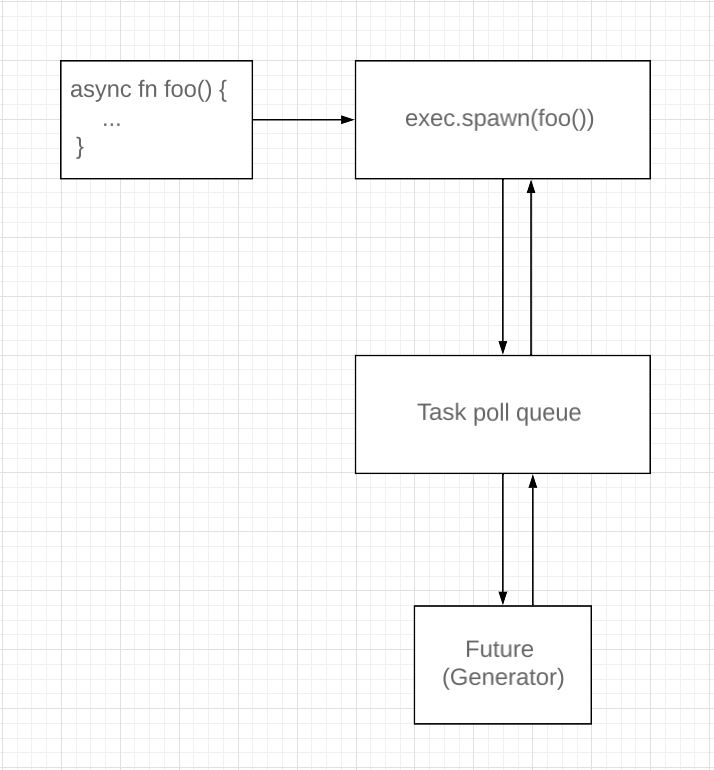
\includegraphics[width=\textwidth,height=6.5cm,keepaspectratio]{images/simple-model.png}
\end{center}
\end{frame}

% ----------------------------------------------------------------- %

\begin{frame}[fragile]
\frametitle{Ideas of Rust's Asynchronous model}
But wait! We're doing a lot of waiting just polling futures one after another! We don't want our CPU do to so much useless work.

Let's add another concept: waker. This function is passed to the future when polling it, and for future it means ``I'll call it when I'll be able to make some progress''.

\begin{minted}[fontsize=\small]{rust}
    trait SimpleFuture {
        type Output;
        fn poll(&mut self, wake: fn()) -> Poll<Self::Output>;
    }
\end{minted}
\end{frame}

% ----------------------------------------------------------------- %

\begin{frame}[fragile]
\frametitle{Ideas of Rust's Asynchronous model}
Therefore, the \texttt{poll} method of our \texttt{AsyncFileRead} will look like this.

\begin{minted}[fontsize=\small]{rust}
    pub struct AsyncFileRead<'a> {
        file_handle: &'a FileHandle,
    }

    impl SimpleFuture for AsyncFileRead<'_> {
        type Output = Vec<u8>;
        fn poll(&mut self, wake: fn()) -> Poll<Self::Output> {
            if self.file_handle.has_data_to_read() {
                Poll::Ready(self.file_handle.read_buf())
            } else {
                self.file_handle.set_readable_callback(wake);
                Poll::Pending
            }
        }
    }
\end{minted}
\end{frame}

% ----------------------------------------------------------------- %

\begin{frame}[fragile]
\frametitle{Ideas of Rust's Asynchronous model}
After this, the model will look like this.

\begin{center}
    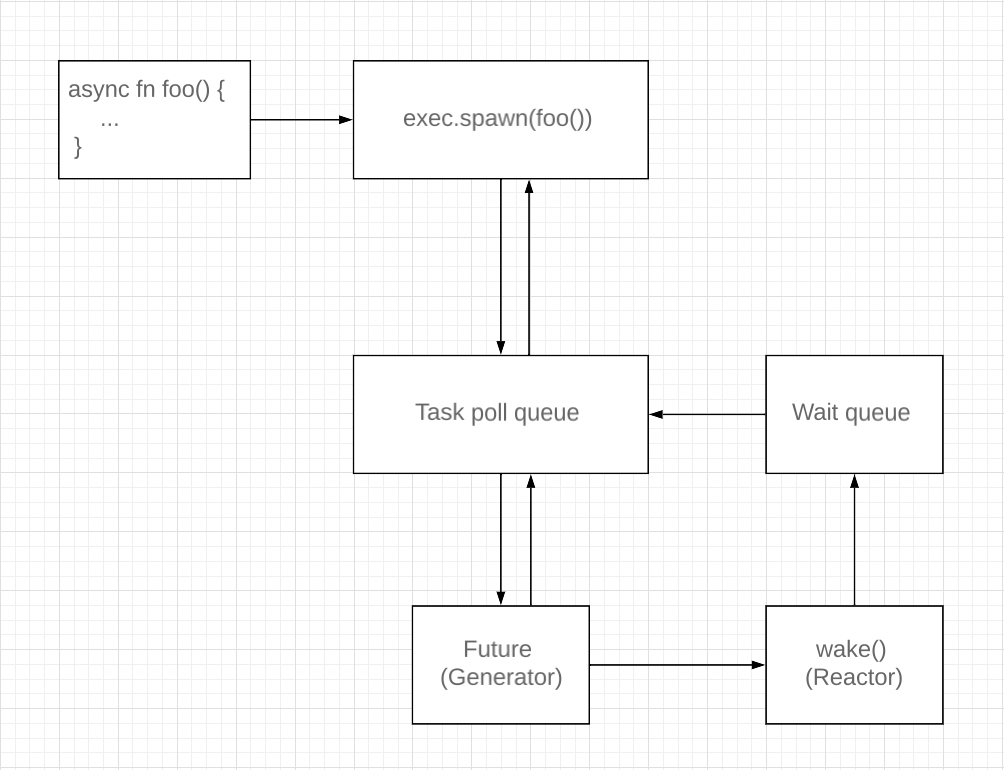
\includegraphics[width=\textwidth,height=7cm,keepaspectratio]{images/real-model.png}
\end{center}
\end{frame}

% ----------------------------------------------------------------- %

\begin{frame}[c]
\centering\Huge\textbf{A real \texttt{Future}: \texttt{Context}}
\end{frame}

% ----------------------------------------------------------------- %

\begin{frame}[fragile]
\frametitle{\texttt{Context}}
You may wonder: ``We only have an \texttt{fn()} pointer. How can we wake ourselfs when we are not the only future executing in the task queue''?
\end{frame}

% ----------------------------------------------------------------- %

\begin{frame}[fragile]
\frametitle{\texttt{Context}}
You may wonder: ``We only have an \texttt{fn()} pointer. How can we wake ourselfs when we are not the only future executing in the task queue''?

The time has come. This \texttt{SimpleFuture} was a lie! Actually, we'll need to store some context about who we are and how we want to be woken. Actually, the \textit{\textbf{true}} \texttt{Future} trait accepts a \texttt{Context} instead of \texttt{fn()}.

\begin{minted}[fontsize=\small]{rust}
    pub trait Future {
        type Output;
        fn poll(
            self: Pin<&mut Self>,
            cx: &mut Context<'_>
        ) -> Poll<Self::Output>;
    }
\end{minted}
\end{frame}

% ----------------------------------------------------------------- %

\begin{frame}[fragile]
\frametitle{\texttt{Context}}
At the same time, \textit{currently}, \texttt{Context} wraps a reference to the \texttt{Waker} type (and this lifetime \texttt{'a} comes from the reference!).

\begin{minted}{rust}
    pub struct Context<'a> { ... }
\end{minted}

The most important functions here:

\begin{minted}{rust}
    pub fn from_waker(waker: &'a Waker) -> Self;

    pub fn waker(&self) -> &'a Waker;
\end{minted}
\end{frame}

% ----------------------------------------------------------------- %

\begin{frame}[fragile]
\frametitle{\texttt{Context}}
\texttt{Waker} is the type which encapsulates \texttt{RawWaker}. Implements \texttt{Clone}, \texttt{Send}, and \texttt{Sync}.

\begin{minted}{rust}
    #[repr(transparent)]
    pub struct Waker { ... }
\end{minted}

The most important functions here:

\begin{minted}{rust}
    // Wakes the associated task
    pub fn wake(self);

    // Constructs a Waker from the RawWaker
    pub unsafe fn from_raw(waker: RawWaker) -> Waker
\end{minted}
\end{frame}

% ----------------------------------------------------------------- %

\begin{frame}[fragile]
\frametitle{\texttt{Context}}
A \texttt{RawWaker} allows the implementor of a task executor to create a \texttt{Waker} which provides customized wakeup behavior. It consists of a pointer to the data and the pointer to the virtual table.

\begin{minted}{rust}
    pub struct RawWaker {
        data: *const (),
        vtable: &'static RawWakerVTable,
    }
\end{minted}

The only important function here is the constructor.

\begin{minted}{rust}
    fn new(
        data: *const (),
        vtable: &'static RawWakerVTable
    ) -> RawWaker;
\end{minted}
\end{frame}

% ----------------------------------------------------------------- %

\begin{frame}[fragile]
\frametitle{\texttt{Context}}
The last structure we must talk about is the \texttt{RawWakerVTable}. It consists of 4 functions, but we'll actually talk about only 3 of them: \texttt{clone}, \texttt{wake} and \texttt{drop}.

\begin{minted}{rust}
    pub const fn new(
        clone: unsafe fn(_: *const ()) -> RawWaker,
        wake: unsafe fn(_: *const ()),
        // Not important currently
        wake_by_ref: unsafe fn(_: *const ()),
        drop: unsafe fn(_: *const ())
    ) -> Self;
\end{minted}
\end{frame}

% ----------------------------------------------------------------- %

\begin{frame}[fragile]
\frametitle{\texttt{Context}}
\begin{itemize}
    \item \texttt{clone} function will be called when the \texttt{RawWaker} gets cloned, e.g. when the Waker in which the \texttt{RawWaker} is stored gets cloned.
    \item \texttt{wake} function will be called when \texttt{wake} is called on the \texttt{Waker}. It must wake up the task associated with this \texttt{RawWaker}.
    \item \texttt{drop} function gets called when a \texttt{RawWaker} gets dropped.
\end{itemize}

The implementations of these functions must retain all resources that are required for this additional instance of a \texttt{RawWaker} and associated task, therefore they are \texttt{unsafe}.
\end{frame}

% ----------------------------------------------------------------- %

\begin{frame}[fragile]
\frametitle{\texttt{Context}}
\textbf{Question}: Why do we need \texttt{Waker} constructor \texttt{from\_raw} to be unsafe?

\visible<2->{
    It's not bad to create a broken \texttt{RawWaker}. It's bad if our runtime will use it!
}

\visible<3->{
    \textbf{Question}: How we'll implement cancelation in Rust's asynchronous model?
}

\visible<4->{
    We'll just stop pulling future when it tries to wake with the canceled state.
}
\end{frame}

% ----------------------------------------------------------------- %

\begin{frame}[fragile]
\frametitle{\texttt{Context}}
For instance, this is a \texttt{RawWaker} that does nothing:

\begin{minted}{rust}
    fn dummy_raw_waker() -> RawWaker {
        fn no_op(_: *const ()) {}
        fn clone(_: *const ()) -> RawWaker {
            dummy_raw_waker()
        }

        let vtable = &RawWakerVTable::new(
            clone, no_op, no_op, no_op
        );
        RawWaker::new(0 as *const (), vtable)
    }
\end{minted}
\end{frame}

% ----------------------------------------------------------------- %

\begin{frame}[c]
\centering\Huge\textbf{Tying It All Together}
\end{frame}

% ----------------------------------------------------------------- %

\begin{frame}[fragile]
\frametitle{Tying It All Together}
It's time to understand our model fully. Let's code a simple asynchronous runtime!

\begin{itemize}
    \item Firstly, we'll try to implement a \texttt{Future}. We'll only build \texttt{TimerFuture}, which will finish after specified time.
    \item Secondly, we'll need some executor that will execute futures, in particular our \texttt{TimerFuture}.
\end{itemize}
\end{frame}

% ----------------------------------------------------------------- %

\begin{frame}[fragile]
\frametitle{Tying It All Together}
As we already know, non-leaf futures just call \texttt{poll} with their's \texttt{waker} on some upstream future. But when we are writing a leaf future, we need to somehow ensure that we'll be woken when ready to make progress.

\visible<2->{
    Usually, asynchronous runtimes like Rust's Tokio provide their own leaf futures and executors, and you're just writing high-level safe code around them using \texttt{async}/\texttt{await}.
}

\visible<3->{
    But we're here studying hardcore Rust, right? Let's build a runtime by ourselfs!
}
\end{frame}

% ----------------------------------------------------------------- %

\begin{frame}[fragile]
\frametitle{Tying It All Together}
Our \texttt{TimerFuture} has a shared state showing whether we're ready or not. It's shared between a sleeping thread (not very efficient, but works!) and our future.

\begin{minted}{rust}
    pub struct TimerFuture {
        // Shared state between the future and
        // the sleeping thread
        state: Arc<Mutex<SharedState>>,
    }

    struct SharedState {
        completed: bool,
        // This is our Waker. If it exists, we'll
        // call wake on it from the sleeping thread
        waker: Option<Waker>,
    }
\end{minted}
\end{frame}

% ----------------------------------------------------------------- %

\begin{frame}[fragile]
\frametitle{Tying It All Together}
\begin{minted}[fontsize=\small]{rust}
    impl Future for TimerFuture {
        type Output = ();
        fn poll(
            self: Pin<&mut Self>, cx: &mut Context<'_>
        ) -> Poll<Self::Output> {
            let mut state = self.state.lock().unwrap();
            if state.completed {
                Poll::Ready(())
            } else {
                // Set waker so that the thread can wake up
                // the current task when the timer has completed
                state.waker = Some(cx.waker().clone());
                Poll::Pending
            }
        }
    }
\end{minted}
\end{frame}

% ----------------------------------------------------------------- %

\begin{frame}[fragile]
\frametitle{Tying It All Together}
Note that clone at the \texttt{Some(cx.waker().clone())} line! It's not efficient, since our \texttt{Waker} may not be changed. For this, there exists \texttt{Waker::will\_wake} function that checks whether two wakers wake the same task.

Now, the last one: actual constructor of the \texttt{Future}.
\end{frame}

% ----------------------------------------------------------------- %

\begin{frame}[fragile]
\frametitle{Tying It All Together}
\begin{minted}[fontsize=\small]{rust}
    impl TimerFuture {
        pub fn new(duration: Duration) -> Self {
            let state = Arc::new(Mutex::new(SharedState {
                completed: false, waker: None,
            }));
            let thread_state = state.clone();
            thread::spawn(move || {
                thread::sleep(duration);
                let mut state = thread_state.lock().unwrap();
                state.completed = true;
                if let Some(waker) = state.waker.take() {
                    waker.wake()
                }
            });
            TimerFuture { state }
        }
    }
\end{minted}
\end{frame}

% ----------------------------------------------------------------- %

\begin{frame}[fragile]
\frametitle{Tying It All Together}
Ok, we've built a future. Now, we need an executor to run the future on.

\begin{minted}[fontsize=\small]{rust}
    struct Executor {
        ready_queue: Receiver<Arc<Task>>,
    }
    // `Spawner` spawns new futures onto the task channel.
    #[derive(Clone)]
    struct Spawner {
        task_sender: Sender<Arc<Task>>,
    }

    type BoxFuture<'a, T> =
        Pin<Box<dyn Future<Output = T> + Send + 'a>>;
    struct Task {
        future: Mutex<Option<BoxFuture<'static, ()>>>,
        task_sender: Sender<Arc<Task>>,
    }
\end{minted}
\end{frame}

% ----------------------------------------------------------------- %

\begin{frame}[fragile]
\frametitle{Tying It All Together}
\begin{minted}[fontsize=\small]{rust}
    impl ArcWake for Task {
        fn wake_by_ref(arc_self: &Arc<Self>) {
            // Implement `wake` by sending this task back
            // onto the task channel, so that it will be
            // polled again by the executor.
            let cloned = arc_self.clone();
            arc_self
                .task_sender
                .send(cloned)
                .expect("too many tasks queued");
        }
    }
\end{minted}
\end{frame}

% ----------------------------------------------------------------- %

\begin{frame}[fragile]
\frametitle{Tying It All Together}

\begin{minted}[fontsize=\small]{rust}
    fn new_executor_and_spawner() -> (Executor, Spawner) {
        let (task_sender, ready_queue) = unbounded_channel();
        (Executor { ready_queue }, Spawner { task_sender })
    }
    impl Spawner {
        fn spawn(
            &self, future: impl Future<Output = ()> + 'static + Send
        ) {
            let future = Box::pin(future);
            let task = Arc::new(Task {
                future: Mutex::new(Some(future)),
                task_sender: self.task_sender.clone(),
            });
            self.task_sender.send(task)
                .expect("channel disconnected");
        }
    }
\end{minted}
\end{frame}

% ----------------------------------------------------------------- %

\begin{frame}[fragile]
\frametitle{Tying It All Together}
\begin{minted}[fontsize=\small]{rust}
    impl Executor {
        fn run(&self) {
            while let Ok(task) = self.ready_queue.recv() {
                let mut future_slot = task.future.lock().unwrap();
                if let Some(mut future) = future_slot.take() {
                    // Create a Waker from the task itself
                    let waker = waker_ref(&task);
                    let context = &mut Context::from_waker(&*waker);
                    if future.as_mut().poll(context).is_pending() {
                        // We're not done processing the future
                        // Put it back to run again later
                        *future_slot = Some(future);
                    }
                }
            }
        }
    }
\end{minted}
\end{frame}

% ----------------------------------------------------------------- %

\begin{frame}[fragile]
\frametitle{Tying It All Together}
\begin{minted}[fontsize=\small]{rust}
    fn main() {
        let (executor, spawner) = new_executor_and_spawner();

        // This Future is non-leaf
        spawner.spawn(async {
            println!("howdy!");
            // And it's a leaf future
            TimerFuture::new(Duration::new(2, 0)).await;
            println!("done!");
        });
        drop(spawner);

        executor.run();
    }
\end{minted}
\end{frame}

% ----------------------------------------------------------------- %

\begin{frame}[c]
\centering\Huge\textbf{Conclusion}
\end{frame}

% ----------------------------------------------------------------- %

\begin{frame}[fragile]
\frametitle{Conclusion}
\begin{itemize}
    \item<1-> Asynchronous computing in Rust works throught the concept of the \texttt{Future}.
    \item<2-> \texttt{Future} is something that is trying to make a progress when \texttt{poll}ed.
    \item<3-> There's leaf and non-leaf futures. The first is provided by the runtime, and the second is created by the user using \texttt{async}/\texttt{await}.
    \item<4-> \texttt{async} is the way to ``color'' a function, marking it as asynchronous.
    \item<5-> \texttt{await} is the keyword to mark the state of the state machine.
    \item<6-> \texttt{await} can make a self-referential structure. To mark the structure self-referential, we use the \texttt{Pin}.
\end{itemize}
\end{frame}

% ----------------------------------------------------------------- %

\begin{frame}[fragile]
\frametitle{Conclusion}
\begin{itemize}
    \item<1-> When you construct the \texttt{Pin}, you promise that you'll never move your type again.
    \item<2-> If your object is \texttt{Unpin}, it means that it doesn't care about the \texttt{Pin} promise.
    \item<3-> If you can, don't give a \texttt{Pin} promise.
    \item<4-> When you try to run the \texttt{Future}, you first \texttt{poll} it.
    \item<5-> Sometimes, \texttt{Future} cannot make progress. Instead of infinite polling, you should put it to the waiting queue.
    \item<6-> And then receive the \texttt{Waker}'s signal to put it to the polling queue.
    \item<7-> User don't need \texttt{Waker}: it's the part of a runtime.
\end{itemize}
\end{frame}

% ----------------------------------------------------------------- %

\begin{frame}
\center\Huge\textbf{See you next time!}


\includegraphics[height=6cm,keepaspectratio]{images/rustacean.png}
\end{frame}

% ----------------------------------------------------------------- %

\end{document}
